\ifnfs
Next version: finir

  \begin{itemize}
    \item CI using median for small sample sizes
    \item RNG
    \item transients
    \item perfect simulation
    \item importance sampling
    \end{itemize}
\fi
%%%%%%%%%%%%%%%%%%%%%%%%%%

\Ifig{simulPilou}{0.95}{0.7}~\\
Simulations are often regarded as the simplest, though most
time consuming performance evaluation method. However, even
simple simulation program may pose problems, if one is not
aware of what stationarity means, and of the potential problems
that arise when a simulation does not have a stationary regime.
We start by discussing this simple, but important issue; the
related topic of freezing simulations is in another chapter
(\sref{sec-freeze}).

Then we describe two commonly used techniques for implementing
a simulation, namely, discrete events and stochastic
recurrences, and discuss how confidence intervals can be
applied to such settings. Then we discuss Monte Carlo
simulation, viewed here as a method for computing integrals or
probabilities, and potential pitfalls about random number
generators. Then we present practical techniques for sampling
from a distribution (CDF inversion, rejection sampling).

Importance sampling is an efficient technique for computing
estimates of rare events, such as a failure rate or a bit error
rate. The main difficulty is the choice of an importance sampling distribution. Here too, we propose a very general approach which is
widely applicable and does not require heavy developments.
%~\\
%~\\
%~\\

\minitoc
\section{What is a Simulation~?}

A simulation is an experiment in the computer (biologists say ``in
silico") where the real environment is replaced by the execution
of a program.
\begin{ex}{Mobile Sensors}
\mylabel{ex-mobile} You want to build an algorithm $A$ for a
system of $n$ wireless sensors, carried by mobile users, which
send information to a central database. A simulation of the
algorithm consists in implementing the essential features of the
program in computer, with one instance of $A$ per simulated
sensor. The main difference between a simulation and a real
implementation is that the real, physical world (here: the radio
channel, the measurements done by sensors) is replaced by events
in the execution of a program.
\end{ex}

\subsection{Simulated Time and Real Time} In a simulation the flow of
time is controlled by the computer. %Let me explain this on an
%example.
A first task of your simulation program is to simulate
parallelism: several parallel actions can take place in the real
system; in your program, you serialize them. Serializing is done
by maintaining a \emph{simulated time}, which is the time at which
an event in the real system is supposed to take place. Every
action is then decomposed into instantaneous events (for example,
the beginning of a transmission), and we assume that it is
impossible that two instantaneous events take place exactly at the
same time.

Assume for example that every sensor in \exref{ex-mobile} should
send a message whenever there is a sudden change in its reading,
and at most every 10 minutes. It may happen in your simulation
program that two or more sensors decide to send a message
simultaneously, say within a window of 10 $\mu$s; your program may
take much more than 10 $\mu$s of \emph{real time} to execute these
events. In contrast, if no event happens in the system during 5
minutes, your simulation program may jump to the next event and
take just of few ms to execute 5 mn of simulated time. The real
time depends on the performance of your computer (processor speed,
amount of memory) and of your simulation program.

\subsection{Simulation Types}
\mylabel{sec-simtypes}
There are many different types of
simulations. We use the following classification.

\paragraph{Deterministic / Stochastic.}
A deterministic simulation has no random components. It is used
when we want to verify a system where the environment is entirely
known, maybe to verify the  feasibility of a schedule, or to test
the feasibility of an implementation.
%
In most cases however, this is not sufficient. The environment of
the system is better modelled with a random component, which makes
the output of the simulation also random.

\paragraph{Terminating / Non-terminating.}
A terminating simulation ends when specific conditions occurs. For
example, if we would like to evaluate the execution time of one
sequence of operations in a well defined environment, we can run
the sequence in the simulator and count the simulated time. A
terminating simulation is typically used when \begin{itemize}
    \item we are interested in the lifetime of some system
    \item or when the inputs are time dependent
\end{itemize}


\begin{ex}{Joe's Computer Shop}
\label{ex-static} We are interested in evaluating the time it
takes to serve $n$ customers who request a file together at time
$0$. We run a simulation program that terminates at time $T_1$
when all users have their request satisfied. This is a terminating
simulation; its output is the time $T_1$.
\end{ex}



\paragraph{Asymptotically Stationary / Non-stationary.}
This applies to a non-terminating, stochastic simulation only.
Stationarity is a property of the stochastic model being
simulated. For an in-depth discussion of stationarity, see
\cref{ch-palm}.

Very often, the state of the simulation depends on the
\imp{initial conditions} and it is difficult to find good
initial conditions; for example, if you simulate an information
server and start with empty buffers, you are probably too
optimistic, since a real server system that has been running
for some time has many data structures that are not empty.
Stationarity is a solution to this problem: if your simulator
has a unique stationary regime, its distribution of state
becomes independent of the initial condition.

A stationary simulation is such that you gain no information
about its age by analyzing it. For example, if you run a
stationary simulation and take a snapshot of the state of the
system at times 10 and 10'000 seconds, there is no way to tell
which of the two snapshots is at time 10 or 10'000 seconds.

In practice, a non terminating simulation is rarely exactly
stationary, but can be \nt{asymptotically stationary}. This means
that after some simulated time, the simulation becomes stationary.

More precisely, a simulation program with time independent inputs
can always be thought of as the simulation of a Markov chain. A
Markov chain is a generic stochastic process such that, in order
to simulate the future after time $t$, the only information we
need is the state of the system at time $t$. This is usually what
happens in a simulation program. The theory of Markov chains (see
\cref{ch-palm}) says that the simulation will either converge to
some stationary behaviour, or will diverge. If we want to measure
the performance of the system under study, it is most likely that
we are interested in its stationary behaviour.

\begin{figure}[!htb]
 \begin{center}
 \subfigure[Utilization = $0.96$]{\ifig{runB}{0.45}}
 \subfigure[Utilization = $1.01$]{\ifig{runC}{0.45}}
 \end{center}
 \mycaption{Simulation of the information server in \exref{ex-sim-des0}, with exponential
 service and interarrival times. The graphs show the number of requests in the queue as a function of time,
 for two values of the utilization factor.}
 \mylabel{fig-simtra}
\end{figure}
%
\begin{ex}{Information Server}
\label{ex-sim-des0} An information server is modelled as a queue.
The simulation program starts with an empty queue. Assume the
arrival rate of requests is smaller than the server can handle.
Due to the fluctuations in the arrival process, we expect some
requests to be held in the queue, from time to time. After some
simulated time, the queue starts to oscillate between busy periods
and idle periods. At the beginning of the simulation, the
behaviour is not typical of the stationary regime, but after a
short time it becomes so (\fref{fig-simtra} (a)).

If in contrast the model is unstable, the simulation output may
show a non converging behaviour (\fref{fig-simtra} (b)).
\end{ex}

In practice, here are the main reasons for non asymptotic
stationarity.\begin{enumerate}
    \item \textbf{Unstable} models: In a
        queuing system where the input rate is larger than the
        service capacity, the buffer occupancy grows unbounded. The longer the simulation is run, the
        larger the mean queue length is.

    \item \textbf{Freezing} simulation: this is a more subtle form
of non stationarity, where the system does not converge to a
steady state but, instead, freezes (becomes slower and slower).
This is typically due to the occurrence of rare events with
large impact. The longer the simulation, the more likely it is
that a rare, but important event occurs, and the larger the
impact of this event may be. If the simulation has regeneration
points (points at which a clean state is reached, for example
when the system becomes empty), then the simulation freezes if
the time interval between regeneration points has an infinite
mean. We study this topic in \sref{sec-freeze}, where we see an
example with the random waypoint.

\item Models with \textbf{seasonal or growth} components, or
    more generally, time dependent inputs;
        for example: internet traffic grows month after month and is more intense at some times of the
        day. %Simulations that incorporate such aspects are
%        terminating simulations, for which the simulation duration
%        is pre-defined.
\end{enumerate}

In most cases, when you perform a non-terminating simulation,
\imp{you should make sure that your simulation is in stationary
regime}. Otherwise, the output of your simulation depends on
the initial condition and the length of the simulation, and it
is often impossible to decide what are realistic initial
conditions. It is not always easy, though, to know in advance
whether a given simulation model is asymptotically stationary.
\cref{ch-palm} gives some examples.
%
%\begin{ex}{Mobile Network}
%\label{ex-mobile} Mobile users communicate via base station, using
%a wireless access scheme. We are interested in the throughput per
%user.
%\end{ex}
%
%In this course: either terminating or non terminating stationary.
\nfs{\paragraph{Why it is Important to Understand Stationarity}
\begin{ex}{Random Waypoint Stationary Distribution}
Put DCC example here.
\end{ex}}
\mq{q-simul-stat19s}
 {Among the following sequences $X_n$ say which ones are
 stationary:
 \begin{enumerate}
 \item $X_n$, $n \geq 1$ is i.i.d.
 \item $X_n$ $n \geq 1$ is drawn as follows. $X_1$ is sampled from a
 given distribution $F()$. To obtain $X_n$, $n \geq 2$ we first flip a coin
 (and obtain $0$ with probability $1-p$, $1$ with probability $p$).
 If the coin returns $0$ we let $X_n=X_{n-1}$; else we let $X_n=$ a new
 sample from the distribution $F()$.
 \item $X_n= \sum_{i=1}^n Z_i$, $n \geq 1$, where $Z_n$, $n
     \geq 1$ is an i.i.d. sequence
 \end{enumerate}
 }
 {1. yes 2. yes: $(X_1,X_2)$ has the same joint distribution as, for example $(X_{10},X_{11})$.  In general
 $(X_{n},X_{n+1},...,X_{n+k})$ has the same distribution for all $n$. This is an example of non-i.i.d., but stationary sequence.
 3. No, in general. For example, if the common
 distribution $F()$ has a finite variance $\sigma^2$,  the variance of $X_n$ is $n \sigma^2$, and grows with $n$, which is contradictory with
 stationarity.}
%%%%%%%%%%%%%%%%%%%%%%%%%%
\section{Simulation Techniques}
%%%%%%%%%%%%%%%%%%%%%%%%%%%
There are many ways to implement a simulation program. We
describe two techniques that are commonly used in our context.

\subsection{Discrete Event Simulation}
\begin{figure}[!htb]\begin{center}
 \subfigure[]{\ifig{des-sim1}{0.5}}
 \subfigure[]{\ifig{des-sim2}{0.5}}
 \subfigure[]{\ifig{des-sim3}{0.8}}
 \end{center}
 \mycaption{(a) Events and
their dependencies for \exref{ex-sim-des}. An arrow indicates that
an event may schedule another one. (b) A possible realization of
the simulation and (c) the corresponding sequence of event
execution. The arrows indicate that the execution of the event
resulted in one or several new events being inserted into the
scheduler.} \mylabel{fig-ex-des1}
\end{figure}

Many computer and communication systems are often simulated
using \nt{discrete event simulation} for example with the ns2
or ns3 simulator \cite{ns3}. It works as follows. The core of
the method is to use a global time \pro{currentTime} and an
\nt{event scheduler}. Events are objects that represent
different transitions; all event have an associated firing
time. The event scheduler is a list of events, sorted by
increasing firing times. The simulation program picks the first
event in the event scheduler, advances \pro{currentTime} to the
firing time of this event, and executes the event. The
execution of an event may schedule new events with firing times
$\geq$\pro{currentTime}, and may change or delete events that
were previously listed in the event scheduler. The global
simulation time \pro{currentTime} \imp{cannot} be modified by
an event. Thus, the simulation time jumps from one event firing
time to the next -- hence the name of discrete event
simulation. In addition to simulating the logic of the system
being modelled, events have to update the counters used for
statistics.


\begin{ex}{Discrete Event Simulation of a Simple Server}
\mylabel{ex-sim-des} A server receives requests and serves them one
by one in order of arrival. The times between request arrivals and
the service times are independent of each other. The distribution of
the time between arrivals has CDF $F()$ and the service time has CDF
$G()$. The model is in fact a \nt{GI/GI/1} queue, which stands for
general independent inter-arrival and service times. An outline of
the program is given below. The program computes the mean response
time and the mean queue length.

{\footnotesize
\paragraph{Classes and Objects} We describe this
example using an object oriented terminology, close to that of the
Java programming language. All you need to know about object
oriented programming to understand this example is as follows. An
object is a variable and a class is a type. For example
\texttt{arrival23} is the name of the variable that contains all
information about the 23rd arrival, it is of the class
\texttt{Arrival}. Classes can be nested, for example the class
\texttt{Arrival} is a sub-class of \texttt{Event}. A method is a
function whose definition depends on the class of the object. For
example, the method \texttt{execute} is defined for all objects of
the class \texttt{Event}, and is inherited by all subclasses such
as \texttt{Arrival}. When the method \texttt{execute} is applied
to the object \texttt{arrival23}, the actions that implement the
simulation of an arrival are executed (for example, the counter of
the number of requests in the system is incremented). \\ }

\textbf{Global Variables and Classes} \noitemsep
\begin{itemize}
\item \pro{currentTime} is the global simulated time;
    it can be modified only by the main program.
\item \pro{eventScheduler} is the list of events, in order of
    increasing time.

\item  An event is an object of the class \pro{Event}. It has an
attribute \pro{firingTime} which is the time at which it is to be
executed. An event can be executed (i.e. the \pro{Event} class has
a method called \pro{execute}), as described later.

There are three \pro{Event} subclasses: an event of the class
\pro{Arrival} represents the actions that occur when a request
arrives; \pro{Service} is when a request enters service;
\pro{Departure} is when a request leaves the system. The event
classes are described in detail later.

\item  The object \pro{buffer} is the FIFO queue of
  Requests. The queue length (in number of
  requests) is \pro{buffer.length}.
  The number of requests served so far is contained in the global variable \pro{nbRequests}.
  The class \pro{Request} is used to describe the requests arriving at the server. At a given point in time,
  there is one
  object of the class \pro{Request} for every request present in the system being modelled. An object of the class
  \pro{Request} has an arrival time attribute.

\item Statistics Counters: \pro{queueLengthCtr} is $\int_0^t
q(s)ds$ where $q(s)$ is the value of \pro{buffer.length} at time
 $s$ and $t$ is the current time. At the end of the simulation, the
mean queue length is \pro{queueLengthCtr}$/T$ where $T$ is the
simulation finish time.

The counter \pro{responseTimeCtr} holds $\sum_{m=1}^m R_m$ where
$R_m$ is the response time for the $m$th request and $n$ is the
value of \pro{nbRequests} at the current time. At the end of the
simulation, the mean response time is \pro{responseTimeCtr}$/N$
where $N$ is the value of \pro{nbRequests}.
\end{itemize}

\textbf{Event Classes. }For each of the three event classes, we
describe now the actions taken when an event of this class is
``executed".
\begin{itemize}
    \item \pro{Arrival}: \emph{Execute Event's Actions}. Create a
    new
    object of class \pro{Request}, with
    arrival time equal to \pro{currentTime}. Queue it at the
    tail of \pro{buffer}.

    \emph{Schedule Follow-Up Events}. If \pro{buffer} was empty before the insertion,
    create a new event of class \pro{Service},
    with the same \pro{firingTime} as this event, and insert it
    into \pro{eventScheduler}.

    Draw a random number $\Delta$ from the distribution $F()$.
    Create a new event of class \pro{Arrival},
    with \pro{firingTime} equal to this event  \pro{firingTime}$+\Delta$,
    and insert it into \pro{eventScheduler}.

    \item \pro{Service}: \emph{Schedule Follow-Up Events}. Draw a
    random number $\Delta$ from the distribution $G()$. Create a new event of class \pro{Departure},
    with \pro{firingTime} equal to this event's
    \pro{firingTime}$+\Delta$,
    and
    insert it into \pro{eventScheduler}.

    \item \pro{Departure}: \emph{Update Event Based Counters}. Let \pro{c} be the request
    at the head of
    \pro{buffer}. Increment \pro{responseTimeCtr} by $d-a$, where
    $d$ is this event's \pro{firingTime} and
    $a$ is the arrival time of the request \pro{c}.
    Increment \pro{nbRequests} by $1$.

    \emph{Execute Event's Actions}. Remove the request \pro{c} from \pro{buffer}
    and delete it.

    \emph{Schedule Follow-Up Events}. If \pro{buffer} is not empty
    after the removal, create a new event of class \pro{Service},
    with \pro{firingTime} equal to this event's
    \pro{firingTime}, and
    insert it into \pro{eventScheduler}.

\end{itemize}

\begin{sh}
\textbf{Main Program}
\begin{itemize}
    \item \emph{Bootstrapping}. Create a new event of class
    \pro{Arrival} with \pro{firingTime} equal to $0$ and insert it into
    \pro{eventScheduler}.
    \item \emph{Execute Events}. While the simulation stopping
    condition is not fulfilled, do the following.
    \begin{itemize}
        \item \emph{Increment Time Based Counters.} Let \pro{e} be
    the first event in \pro{eventScheduler}. Increment
     \pro{queueLengthCtr} by $q (t_{\mathrm{new}}-
     t_{\mathrm{old}})$
    where $q=$\pro{buffer.length},
    $t_{\mathrm{new}}$=\pro{e.firingTime}
    and $t_{\mathrm{old}}=$\pro{currentTime}.
        \item Execute \pro{e}.
        \item Set \pro{currentTime} to \pro{e.firingTime}
        \item Delete \pro{e}
    \end{itemize}
\item \emph{Termination}. Compute the final statistics:\\
\pro{meanQueueLength}=\pro{queueLengthCtr}/\pro{currentTime}\\
 \pro{meanResponseTime}=\pro{responseTimeCtr}/\pro{nbRequests}
\end{itemize}
\end{sh}

\fref{fig-ex-des1} illustrates the program.
\noitemsep
\end{ex}



\mq{q-stat-2}{Can consecutive events have the same firing
time~?}{Yes. In \exref{ex-sim-des}, a \pro{Departure} event when
the queue is not empty is followed by a \pro{Service} event with
the same firing time.}

\mq{q-stat-sim2}{What are the generic actions that are executed
when an event is executed~? }{1. Update Event Based Counters 2.
Execute Event's Actions 3. Schedule Follow-Up Events.}

\mq{q-stat-sim22}{Is the model in \exref{ex-sim-des}
stationary~? }{It depends on the parameters. Let $a$ [resp.
$b$] be the mean of $F()$ [resp. $G()$]. The utilization factor
of the queue is $\rho=\frac{b}{a}$. If $\rho <1$ the system is
stable and thus asymptotically stationary, else not (see
\cref{ch-queuing}).}

\mq{q-stat-1}{Is the mean queue length an event-based or a
time-based statistic~? The mean response time~?}{Mean queue
length: time based. Mean response time: event based.}

%\mq{q-stat-sim3}{What is the difference between an event based
%counter and a time based counter~? What statistics are they used
%for~?}{An event based counter is updated when an event is
%executed1. A time based counter is updated when the current time
%changes. The former are used for event based a Update Event Based
%Counters 2. Execute Event's Actions 3. Schedule Follow-Up Events.}

\subsection{Stochastic Recurrence}
\begin{figure}[!htb]
\begin{center}
 \subfigure[1 mobile]{\ifig{rwp1}{0.7}}\\
 \subfigure[10 mobiles]{\ifig{rwp2}{0.7}}
\end{center}
 \mycaption{Simulation of the random waypoint model.}
 \mylabel{fig:rwp1}
\end{figure}
%
\mylabel{sec-stocrec} This is another simulation method; it is
usually much more efficient than discrete event simulation, but
requires more work on the model. A \nt{stochastic recurrence}
is a recurrence of the form:
 \be
 \bracket{
 X_0=x_0\\
  X_{n+1}=f(X_n,Z_n)
  }
  \mylabel{eq-sr}
 \ee
 where $X_n$ is the state of the system at the $n$th transition
 ($X_n$ is in some arbitrary state space
$\calX$), $x_0$ is a fixed, given state in $\calX$, $Z_n$ is
some stochastic process that can be simulated (for example a
sequence of i.i.d. random variables, or a Markov chain), and
$f$ is a deterministic mapping. The simulated time $T_n$ at
which the $n$th transition occurs is assumed to be
 included in the state variable
 $X_n$.

 \begin{ex}{Random Waypoint}
 \mylabel{ex-rwp-sim}

The \nt{random waypoint} is a model for a mobile point, and can be
used to simulate the mobility pattern in \exref{ex-mobile}. It is
defined
 as follows. The state variable is $X_n=(M_n, T_n)$ where $M_n$ is
 the position of the mobile at the $n$th transition (the $n$th
 ``waypoint") and $T_n$ is the time at which this destination is
 reached. The point $M_n$ is chosen at random, uniformly in a given convex area
 $\calA$. The speed at which the mobile travels to the next
 waypoint is also chosen at random uniformly in
 $[v_{\min},v_{\max}]$.

 The random waypoint model can be cast as a stochastic recurrence
 by letting $Z_n=(M_{n+1},V_{n+1})$, where $M_{n+1},V_{n+1}$ are independent
 i.i.d. sequences, such that $M_{n+1}$ is uniformly distributed in
 $\calA$ and $V_{n+1}$ in $[v_{\min},v_{\max}]$. We have then the
 stochastic recurrence
  \ben
  X_{n+1}:=(M_{n+1},T_{n+1}) = (M_{n+1}, T_n + {\|M_{n+1}-M_n\|\over V_n})
  \een
  See \fref{fig:rwp1} for an illustration.
\end{ex}


 Once a system is cast as a stochastic recurrence, it
can be simply simulated as a direct implementation of
\eref{eq-sr}, for example in Matlab.

\mq{q-sim-kwsd}{Is the random waypoint model asymptotically
stationary~?}{For $v_{\min}>0$ it is asymptotically stationary.
For $v_{\min}=0$ it is not: the model ``freezes" (the number of
waypoints per time unit tends to $0$). See \cref{ch-palm} for a
justification).}

\paragraph{Stochastic Recurrence Versus Discrete Event Simulation}
It is always possible to express a stochastic simulation as a
stochastic recurrence, as illustrated by the next example. Both
representations may have very different memory and CPU
requirements; which representation is best depends on the
problem at hand.

\begin{ex}{Simple Server as a Stochastic Recurrence} (Continuation of
\exref{ex-sim-des}). Consider implementing the simple server in
\exref{ex-sim-des} as a stochastic recurrence. To simplify,
assume we are interested only in the mean queue length and not
the mean response time. This can be implemented as a stochastic
recurrence as follows.
%
Let $X_n = (t_n, b_n,q_n,a_n,d_n)$ represent the state of the
simulator just \emph{after} an arrival or a departure,
%, as
%follows:
%
% \ben
% X_n = (t_n, b_n,q_n,a_n,d_n)
% \een
 $t_n=$ the simulated time at which this transition occurs,
 $b_n=$\pro{buffer.length},  $q_n=$ \pro{queueLengthCtr}
 (both just after the transition), $a_n=$ the time interval from this transition to
 the next arrival and $d_n$= the time interval from this transition to
 the next departure.

Let $Z_n$ be a couple of two random numbers, drawn independently
of anything else, with distribution uniform in $(0,1)$.

The initial state is
 \ben
 t_0=0, \; b_0=0, \;q_0=0, \; a_0=F^{-1}(u),\;d_0=\infty
 \een
 where $u$ is a sample of the uniform distribution on $(0,1)$. The
 reason for the formula $a_0=F^{-1}(u)$ is explained in
 \sref{sec-arbdis}: $a_0$ is a sample of the distribution with CDF
 $F()$.

 The recurrence is defined by $f((t,b,q,a,d),(z_1,z_2))=(t',b',q',a',d')$ with
 \bearn
\lefteqn{\mif a < d  \mbox{  // this transition is an arrival}}\\
&& \Delta = a\\
&&t'= t + a\\
&&b'=b+1\\
&&q'= q + b  \Delta\\
&&a'=F^{-1}(z_1)\\
&&\mif b==0 \mthen d'= G^{-1}(z_2) \melse  d'=d-\Delta\\
\lefteqn{\melse \mbox{  // this transition is a departure}}\\
&& \Delta = d\\
&&t'= t + d\\
&&b'=b-1\\
&&q'= q + b  \Delta\\
&&a'=a-\Delta\\
&&\mif b' > 0 \mthen d'=G^{-1}(z_1) \melse d'=\infty\\
 \eearn
\end{ex}

\section{Computing the Accuracy of Stochastic Simulations}
\mylabel{stats-sim} A simulation program is expected to output
some quantities of interest. For example, for a simulation of the
algorithm $A$ it may be the average number of lost messages. The
output of a stochastic simulation is random: two different
simulation runs produce different outputs. Therefore, it is not
sufficient to give one simulation result; in addition, we need to
give the accuracy of our results.

\subsection{Independent Replications}
A simple and very efficient method to obtain confidence intervals
is to use \nt{replication}. Perform $n$ independent replications
of the simulation, each producing an output $x_1, ...,x_n$. \imp{Be careful to have truly random seeds} for the random number
generators, for example by accessing computer time
(\sref{sec:rng}).

\subsection{Computing Confidence Intervals}
You have to choose whether you want a confidence interval for the
median or for the mean. The former is straightforward to compute,
thus should be preferred in general.

Methods for computing confidence intervals for median and mean
are summarized in \sref{sec-conf-cimean}.
\begin{ex}{Application to \exref{ex-static}} \fref{fig-ex-static}
shows the time it takes to transfer all files as a function of the number
of customers. The simulation outputs do not appear to be normal,
therefore we test whether $n$ is large, by looking at the qqplot
of the bootstrap replicates. We find that it looks normal, and we
we can therefore use the Student statistic. Out of curiosity, we also compute
the bootstrap percentile estimate and find that both confidence
intervals are very close, the bootstrap percentile estimate being
slightly smaller.
\end{ex}
\begin{figure}[!htb]
\begin{center}
 \subfigure[]{\Ifignc{sim-raw}{0.49}{0.4}}
 \subfigure[]{\Ifignc{sim-conf}{0.49}{0.4}}
 \subfigure[]{\Ifignc{sim-qqplots}{0.49}{0.4}}
 \subfigure[]{\Ifignc{sim-qqbs}{0.49}{0.4}}

\end{center} \mycaption{Time to serve $n$ files in Joe's computer
shop (\exref{ex-static}): (a) results of 30 independent
replications, versus number of customers (b) 95\%confidence
intervals for the mean obtained with the normal approximation
(left), with the bootstrap percentile estimate (middle); 95\%
confidence interval for the median (right). (c) qqplot of
simulation outputs, showing deviation from normality (d) qq-plots
of the bootstrap replicates, showing normality.}
\mylabel{fig-ex-static}
\end{figure}


There are other methods of obtaining confidence intervals, but
they involve specific assumptions on the model and require some
care; see for example \cite{law2000simulation}.

\subsection{Non-Terminating Simulations}
Non-terminating simulations should be asymptotically stationary
(\sref{sec-simtypes}). When you simulate such a model, you should
be careful to do \nt{transient removal}. This involves
determining:
\begin{itemize}
    \item when to start measuring the output (this is the time at
    which we consider that the simulation has converged to its
    stationary regime
    \item when to stop the simulation
\end{itemize}
%
Unfortunately, there is no simple, bullet proof method to
determine these two times. In theory, convergence to the
stationary regime is governed by the value of the second
eigenvalue modulus of the transition matrix of the markov chain
that represents your simulation. In all but very special cases,
it is impossible to estimate this value. A practical method for
removing transients is to look at the data produced by the
simulation, and visually determine a time after which the
simulation output does not seem to exhibit a clear trend
behaviour. For example, in \fref{fig-simtra} (a), the
measurements could safely start at time  $t=1$. This is the
same stationarity test as with time series
(\cref{ch-forecast}).

Determining when to stop a simulation is more tricky. The
simulation should be large enough for transients to be
removable. After that, you need to estimate whether running the
simulation for a long time reduces the variance of the
quantities that you are measuring. In practice, this is hard to
predict a priori. A rule of thumb is to run the simulation long
enough so that the output variable looks gaussian across
several replications, but not longer.

\nfs{Show very short simulation runs with random waypoint --
illustrate the problem of 1) confidence intervals and 2) need to
remove transients.}
%
%
%\subsection{Avoiding Transients At All (Perfect Simulation)}
%\mylabel{simul-nt} This is possible when the simulation has the
%form of a stochastic recurrence (\sref{sec-stocrec}), and it is
%possible to compute the stationary distribution (i.e. the
%distribution seen at an arbitrary point in time) of the state of
%the system \emph{and} the time until the next transition. This is
%usually done using the inversion formula of Palm calculus
%(\thref{theo-inversion} on \pgref{theo-inversion}). We explain
%this on an example.
%
%\begin{ex}[Perfect Simulation of Random Waypoint]
%TBD
%\end{ex}
%
%Alternative: run the model.
%
%Example de Jorg.
%
%Synchroniser avec chapitre Palm Calculus.
\section{Monte Carlo Simulation}
\mylabel{sec-montecarlo}
 \nt{Monte Carlo simulation} is a method for computing probabilities, expectations, or, in general, integrals
 when direct evaluations is impossible or too complex. It simply consists in estimating the expectation as the mean
 of a number of independent replications.

Formally, assume we are given a model for generating a data
sequence $\vec{X}$. The sequence may be i.i.d. or not. Assume
we want to compute
 $\beta=\E\left(\varphi(\vec{X})\right)$.  Note that this covers the case
 where we want to compute a probability: if $\varphi(\vec{x})=\ind{\vec{x}\in A}$ for some set
 $A$, then $\beta=\P(\vec{X} \in A)$.

Monte-Carlo simulation consists in generating $R$ i.i.d.
replicates $\vec{X}^r$, $r=1,...,R$. The Monte-Carlo estimate
of $\beta$ is
 \be
 \hat{\beta} = \frac{1}{R}\sum_{r=1}^R\varphi(\vec{X}^r)
 \ee

A confidence interval for $\beta$ can then be computed using
the methods in \cref{ch-conf} (\thref{theo-conf-ln} and
\thref{theo-est-proba}). By adjusting $R$, the number of
replications, we can control the accuracy of the
 method, i.e. the width of the confidence interval.

In particular, the theorem for confidence intervals of success
probabilities (\thref{theo-est-proba}) should be used when the
goal is to find an upper bound on a rare probability and the
Monte Carlo estimate returns $0$, as illustrated in the example
below.

 %
 \begin{ex}{$p$-value of a test} Let $X_1, ...,X_n$ be a sequence of i.i.d. random
 variables that take values in the discrete set $\{1,2,...,I\}$. Let $q_i=\P(X_k=i)$.
 Let $N_i=\sum_{k=1}^n \ind{X_k=i}$
(number of observation that are equal to $i$). Assume we want to
compute
 \be p=\P\left(
\sum_{i=1}^k N_i
 \ln\frac{N_i}{n q_i} >a
 \right)
 \ee
 where $a>0$ is given. This computation arises in the theory of goodness of fit tests, when
 we want to test whether $X_i$ does indeed come from the model
 defined above ($a$ is then equal to $\sum_{i=1}^k n_i
 \ln\frac{n_i}{n q_i}$ where $n_i$ is our data set). For large values of the sample size $n$ we can approximate $\beta$
 by a $\chi^2$ distribution (see \sref{sec-lrs-asymptotic}), but
 for small values there is no analytic result.

We use Monte-Carlo simulation to compute $p$. We generate $R$
i.i.d. replicates $X_1^r, ...,X_n^r$ of the sequence
($r=1,...,R$). This can be done by using the inversion method
described in this chapter. For each replicate $r$, let
 \be
 N_i^r=\sum_{k=1}^n \ind{X_k^r=i}
 \ee
 The Monte Carlo estimate of $p$ is
 \be
 \hat{p}=\frac{1}{R} \sum_{r=1}^R \ind{\sum_{i=1}^k N_i
 \ln\frac{N_i}{n q_i} >a}
 \ee

 Assuming that $\hat{p}R \geq 6$, we compute a confidence interval
 by using the normal approximation in \eref{eq-ci-p-dasksadlk}.
 The sample variance is estimated by
 \be
 \hat{\sigma}=\sqrt{\frac{\hat{p}(1-\hat{p})}{R}}
 \ee
 and a confidence interval at level $0.95$ is
 $\hat{p}\pm 1.96\hat{\sigma}$. Assume we want a \imp{relative} accuracy at least equal to some fixed value
 $\epsilon$ (for example $\epsilon=0.05$). This is achieved if
 \be
\frac{1.96\hat{\sigma}}{\hat{p}} \leq \epsilon
 \ee
which is equivalent to
 \be
 \mylabel{eq-acc-mc}
R \geq \frac{3.92}{\epsilon^2}\left(\frac{1}{\hat{p}}-1\right)
 \ee
We can test for every value of $R$ whether \eref{eq-acc-mc} is
verified and stop the simulation when this happens.
\tref{tab-simul-mendel} shows some results with $n=10 0$ and
$a=2.4$; we see that $p$ is equal to 0.19 with an accuracy of
$5\%$; the number of Monte Carlo replicates is proportional to
the relative accuracy to the power $-2$.

If $\hat{p}R< 6$ then we cannot apply the normal approximation.
This occurs when the $p$-value to be estimated is very small.
In such cases, typically, we are not interested in an exact
estimate of the $p$-value, but we want to know whether it is
smaller than some threshold $\alpha$ (for example $\alpha=
0.05$). \eref{eq-ci-p-u} and \eref{eq-ci-p-ksjsda} can be used
in this case. For example, assume the same data as in
\tref{tab-simul-mendel} except for $a=18.2$. We do $R=10^4$
monte carlo replicates and find $\hat{p}R = 0$. We can
conclude, with confidence $95\%$, that $p\leq 1 - \lp
0.025\rp^{1 \over R}=3.7E-4$.


\mylabel{sec-montecarlo-pvalue}
\end{ex}
\begin{table}
\center\begin{tabular}{|c|c|c|}
  % after \\: \hline or \cline{col1-col2} \cline{col3-col4} ...
  \hline
  $R$ & $\hat{p}$ & margin \\ \hline \hline
  30 & 0.2667 & 0.1582 \\
  60 & 0.2500 & 0.1096 \\
  120 & 0.2333 & 0.0757 \\
  240 & 0.1917 & 0.0498 \\
  480 & 0.1979 & 0.0356 \\
  960 & 0.2010 & 0.0254 \\
  1920 & 0.1865 & 0.0174 \\
  3840 & 0.1893 & 0.0124 \\
  7680 & 0.1931 & 0.0088 \\ \hline
\end{tabular}
\mycaption{Computation of $p$ in \exref{sec-montecarlo-pvalue} by
Monte Carlo simulation. The parameters of the model are $I=4$,
$q_1=9/16, q_2=q_3=3/16$, $q_4=1/16$, $n=100$ and $a=2.4$. The table
shows the estimate $\hat{p}$ of $p$ with its $95\%$ confidence
margin versus the number of Monte-Carlo replicates $R$. With 7680
replicates the relative accuracy (margin/$\hat{p}$) is below $5\%$.}
\mylabel{tab-simul-mendel}
\end{table}
\mq{q-klaklddf}{In the first case of
\exref{sec-montecarlo-pvalue} (\tref{tab-simul-mendel}), what
is the conclusion of the test ? In the second case ?}{In the
first case we accept the null hypothesis, i.e. we believe that
the probability of case $i$ is $q_i$. In the second case, the
$p$-value is smaller than $0.05$ so we reject the null
hypothesis.}


\section{Random Number Generators} \mylabel{sec:rng}
 \nfs{Faire une simu avec 2 RNGs differents et comparer
les intervalles de confiance (voir Arsic)}

The simulation of any random process uses a basic function (such
as \pro{rand} in Matlab) that is assumed to return independent
uniform random variables. Arbitrary distributions can be derived
from there, as explained in \sref{sec-arbdis}.

In fact, \pro{rand} is a \nt{pseudo-random number generator}. It
produces a sequence of numbers that appear to be random, but is in
fact perfectly deterministic, and depends only on one
initialization value of its internal stated, called the \nt{seed}.
There are several methods to implement pseudo random number
generators; they are all based on chaotic sequences, i.e.
iterative processes where a small difference in the seed produces
very different outputs.

Simple random number generators are based on \nt{linear
congruences} of the type $ x_n = a x_{n-1} \mod m $. Here the
internal state after $n$ calls to \pro{rand} is the last output
$x_n$; the seed is $x_0$. Like for any iterative algorithm, the
sequence is periodic, but for appropriate choices of $a$ and
$m$, the period may be very large.

\begin{ex}{Linear Congruence}\mylabel{ex-lcg}
A widespread generator (for example the default in ns2) has
$a=16'807$ and $m=2^{31}-1$. The sequence is $x_n= \frac{s a^n
\mod m}{m}$ where $s$ is the seed. $m$ is a prime number, and
the smallest exponent $h$ such that $a^h=1 \mod m$ is $m-1$. It
follows that for any value of the seed $s$, the period of $x_n$
is exactly $m-1$. \fref{fig-rng0} shows that the sequence $x_n$
indeed looks random.
\end{ex}
\begin{figure}
 \begin{center}
 \subfigure[]{\Ifignc{rng-qq}{0.6}{0.3}}
 \subfigure[]{\Ifignc{rng-acf}{0.6}{0.3}}
 \subfigure[]{\Ifignc{rng-lag}{0.6}{0.6}}
 \end{center}%
 \nfs{rngTest.m}
 \mycaption{$1 000$ successive numbers for the generator in \exref{ex-lcg}.
 (a) QQplot against the uniform distribution in $(0,1)$, showing a perfect match.
 (b) autocorrelation function, showing no significant correlation at any lag
 (c) lag plots at various lags, showing independence.}
 \mylabel{fig-rng0}
\end{figure}


The period of a random number generator should be much larger
than the number of times it is called in a simulation. The
generator in \exref{ex-lcg} has a period of ca. $2 \times
10^9$, which may be too small for very large simulations. There
are other generators with much longer periods, for example the
``Mersenne Twister" \cite{matsumoto1998mersenne} with a period
of $2^{19937}-1$. They use other chaotic sequences and
combinations of them.

\begin{figure}[!htb]
\begin{center}
 \subfigure[Linear Congruence with $a=16'807$ and $m=2^{31}-1$]{\ifig{sim-rng1}{0.4}}
 \subfigure[L'Ecuyer"'s generator \cite{l2001software}]{
 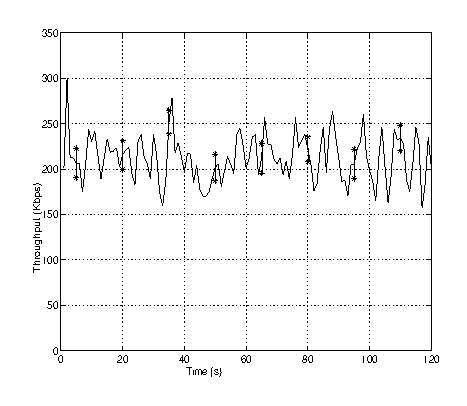
\includegraphics[width=0.4\textwidth,height=0.275\textwidth]{sim-rng2.eps}
 }
\end{center}
\mycaption{Simulation outputs for the throughput of TCP
connections over a wireless ad-hoc network. The wireless LAN
protocol uses random numbers for its operation. This simulation
consumes a very large number of calls to \pro{rand}. The
simulation results obtained with both generators are different:
Lecuyer's generator produces consistently smaller confidence
intervals.}
 \mylabel{fig-rng}
\end{figure}
Perfect pseudo-random number generators do not exist; only
truly random generators can be perfect. Such generators exist:
for example, a quantum mechanics generator is based on the fact
that the state of a photon is believed to be truly random. For
a general text on random number, see \cite{l1998random}; for
software implementing good generators, see \cite{l2001software}
and L'Ecuyer's home page. For a general discussion of
generators in the framework of simulation, see
\cite{hechenleitner1000shortcomings}. \fref{fig-rng}
illustrates a potential problem when the random number
generator does not have a long enough period.


\paragraph{Using a Random Number Generator in Parallel Streams}
For some (obsolete) generators as in \exref{ex-lcg}, choosing
small seed values in parallel streams may introduce a strong
correlation (whereas we would like the streams to be independent).
\begin{ex}{Parallel Streams with Incorrect Seeds}
Assume we need to generate two parallel streams of random numbers.
This is very frequent in discrete event simulations; we may want
to have one stream for the arrival process, and a second one for
the service process. Assume we use the linear congruential
generator of \exref{ex-lcg}, and generate two streams $x_n$ and
$x'_n$ with seeds $s=1$ and $s'=2$. \fref{fig-rng2} shows the
results: we see that the two streams are strongly correlated. In
contrast, taking $s'=$ the last value $x_N$ of the first stream
does not have this problem.

More modern generators as mentioned above do not have this problem
either.
\end{ex}
\begin{figure}[!htb]
 \begin{center}
 \subfigure[]{\Ifignc{rng-2str}{0.7}{0.3}}
 \subfigure[]{\Ifignc{rng-2str-ren}{0.7}{0.3}}
 \end{center}%
\nfs{rng.m}
 \mycaption{$x_n$ versus $x'_n$ for two streams
generated with the linear congruential in \exref{ex-lcg}. (a) seed
values are 1 and 2 (b) seed values are (1, last value of first
stream).}
 \mylabel{fig-rng2}
\end{figure}

\paragraph{Seeding the Random Number Generator}
A safe way to make sure that replications are reasonably
independent is to use the internal state of the generator at the
end of the 1st replication as seed for the second replication and
so one. This way, if the generator has a long enough sequence, the
different replications have non overlapping sequences.

In practice, though, we often want independent replications to
be run in parallel, so this mode of operation is not possible.
A common practice is to take as seed a truly random number, for
example derived from the computer clock or user input with the
mouse.

\section{How to Sample from a Distribution}
\mylabel{sec-arbdis}\nfs{\begin{itemize}
    \item methode inversion cas simples
    \item methode de sampling $(X,U)$ conditional to $U< f(x)$
    (Ycart Propositions 2.5 et 2.6)
    \item Simulation of normal random variables (graphique)
    \item ad-hoc methods : permutation
    \item conditional law
\end{itemize}
} In this section we discuss methods to produce a sample $X$
for a random variable that has a known distribution. We assume
that we have a random number generator, that provides us with
independent samples of the uniform distribution on $(0,1)$. We
focus on two methods of general applicability: CDF inversion
and rejection sampling.

\subsection{CDF Inversion}
The method of \nt{CDF inversion}, also called
\nt{percentile inversion method}, applies to real
or integer valued random variable, when the CDF
is easy to invert.
\begin{shadethm}
Let $F$ be the CDF of a random variable $X$ with values in $\Reals$.
Define the \nt{pseudo-inverse}, $F^{-1}$ of $F$ by
 \ben
 F^{-1}(p)= \sup \{x: F(x) \leq p\}
 \een
 Let $U$ be a sample of a random variable with uniform distribution on
 $(0,1)$; $F^{-1}(U)$ is a sample of $X$. \label{theo-cdf-inversion}
\end{shadethm}

\imp{Application to real random variable. }In the case where
$X$ has a positive density over some interval $I$, then $F$ is
continuous and strictly increasing on $I$, and the
pseudo-inverse is the inverse of $F$, as in the next example.
It is obtained by solving for $x$ in the equation $F(x)=p$,
$x\in I$.
\begin{ex}{Exponential Random Variable}
The CDF of the \nt{exponential distribution} with parameter
$\lambda$ is $F(x)=1- e^{-\lambda x}$. The pseudo-inverse
(which in this case is the plain inverse) is obtained by
solving the equation \ben 1- e^{-\lambda x} = p \een where $x$
is the unknown. The solution is $x=- \frac{\ln
(1-p)}{\lambda}$. Thus a sample $X$ of the exponential
distribution is obtained by letting $X = - \frac{\ln
(1-U)}{\lambda}$, or, since $U$ and $1-U$ have the same
distribution:
  \be
X = - \frac{\ln (U)}{\lambda}
 \mylabel{eq-gen-exp}
  \ee
  where $U$ is the output of the random number generator.
\end{ex}

\imp{Application to integer random variable. } Assume $N$ is a
random variable with values in $\Nats$. Let $p_k=\P(N=k)$, then for
$n\in \Nats$:
 \ben
 F(n) = \sum_{k=0}^n p_k
 \een
and for $x \in \Reals $:
 \ben \bracket{\mif x <0 \mthen F(x) = 0 \\
 \melse F(x)= \P(N\leq x)=\P(N \leq \lfloor x \rfloor) = F(\lfloor x
 \rfloor)
 }
 \een
 We now compute $F^{-1}(p)$, for $0<p<1$. Let $n$ be the smallest
 integer such that $p<F(n)$. The set $\{x : F(x) \leq p\}$ is equal
 to $(-\infty, n)$ (\fref{fig-pseudo-inverse}); the supremum of this set is $n$,
 thus $F^{-1}(p)=n$. In other words, the pseudo inverse is given by
 \be
F^{-1}(p) = n \Leftrightarrow F(n-1)  \leq p <F(n)
\mylabel{eq-pi-int}
 \ee
 \begin{figure}[!htb]
 \Ifig{pseudo-inverse}{0.7}{0.4}
 \mycaption{Pseudo-Inverse of CDF $F()$ of an integer-valued random variable}
\mylabel{fig-pseudo-inverse}
 \end{figure}
 Thus we have shown:
  \begin{corollary} Let $N$ be a random variable with values in
  $\Nats$ and let $p_k=\P(N=k)$, for $k \in \Nats$. A sample of
  $N$ is obtained by setting $N$ to the unique index $n\geq 0$
  such that $\sum_{k= 0}^{n-1}p_k \leq U < \sum_{k= 0}^n p_k$,
  where $U$ is the output of the random number generator.
  \end{corollary}
\begin{ex}{Geometric Random Variable}
Here $X$ takes integer values $0,1,2,...$. The \nt{geometric
distribution} with parameter $\theta$ satisfies $\P(X=k)=\theta
(1-\theta)^k$, thus for $n \in \Nats$:
 \ben
 F(n) = \sum_{k=0}^n \theta (1-\theta)^k = 1-(1-\theta)^{n+1}
 \een
by application of \eref{eq-pi-int}:
 \ben
F^{-1}(p)=n \Leftrightarrow n \leq \frac{\ln(1-p)}{\ln(1 -\theta)} <
n+1
 \een
hence
 \ben
F^{-1}(p)=\left\lfloor
 \frac{\ln(1-p)}{\ln(1-\theta)}
 \right\rfloor
 \een
and, since $U$ and $1-U$ have the same distribution, a sample $X$ of
the geometric distribution is
 \be
X=\left\lfloor
 \frac{\ln(U)}{\ln(1-\theta)}
 \right\rfloor
 \mylabel{eq-gen-geom}
 \ee \label{ex-gen-geom}
\end{ex}
\mq{q-sim-lsj5}{Consider the function defined by \pro{COIN(p)=
if rand()<p 0 else 1}. What does it compute~?}{It generates a
sample of the Bernoulli random variable that takes the value
$0$ with $p$ and the value $1$ with  probability $1-p$.}

\mq{q-simul-dklskldaskl90}
 {Compare \eref{eq-gen-exp} and \eref{eq-gen-geom}.
}
 {They are similar, in fact we have $N=\lfloor X\rfloor$ if we let
 $\lambda=\ln(1-\theta)$. This follows from the fact that if
 $X\sim$ exp$(\lambda)$, then $\lfloor X\rfloor$ is geometric
 with parameter $\theta=1-e^{-\lambda}$
}

\subsection{Rejection Sampling}
\label{sec-rej-samp}

The method of \nt{rejection sampling} is widely
applicable. It can be used to generate samples of
random variables when the inversion method does
not work easily. It applies to random vectors of
any dimension.

The method is based on the following result, which is of
independent interest. It allows to sample from a distribution
given in conditional form.
\begin{shadethm}[Rejection Sampling for a Conditional Distribution]
\mylabel{theo-rj1} Let $X$ be a random variable in some space $S$
such that the distribution of $X$ is the conditional distribution
of $\tilde{X}$ given that $\tilde{Y}\in \calA$, where
$(\tilde{X},\tilde{Y})$ is a random variable in $S \times S'$ and
$\calA$ is a measurable subset of $S$.

A sample of $X$ is obtained by the following algorithm:
\begin{tabbing}
  MMMMMMMMM \= MM \=  \kill
  % \> for next tab, \\ for new line...
  \>\textbf{do}  \\
  \>  \> draw a sample of  $(\tilde{X},\tilde{Y})$   \\
  \>\textbf{until} $\tilde{Y} \in \calA$ \\
  \>\textbf{return}($\tilde{X})$
\end{tabbing}

The expected number of iterations of the algorithm is
$\frac{1}{\P(\tilde{Y}\in \calA)}$. \label{theo-simul-rs}
\end{shadethm}


\begin{ex}{Density Restricted to Arbitrary Subset}\mylabel{ex-gen-cond}
Consider a random variable in some space ($\Reals, \Reals^n,
\Ints...$) that has a density $f_Y(y)$. Let $\calA$ be a set such
that $\P(Y \in \calA)>0$. We are interested in the distribution of
a random variable $X$ whose density is that of $Y$, restricted to
$\calA$:
 \be
 \mylabel{eq-dens-cond}
 f_X(y) = K f_Y(y) \ind{y \in \calA}
 \ee
 where $K^{-1}=\P(Y \in \calA)>0$ is a normalizing constant. This
 distribution is the conditional distribution of $Y$, given that
 $Y\in \calA$.
 \mq{q-simul-sadkdskak}{Show this.}{For any (measurable) subset $\calB$ of the space,
 $\P(X\in \calB ) = K \int_{\calB} f_Y(y) \ind{y \in \calA} dy$
 $=K \P(Y\in \calA \mand Y\in \calB)=\P(Y \in \calB|Y\in \calA)$.}

Thus a sampling method for the distribution with density in
\eref{eq-dens-cond} is to draw samples of the  distribution with
density $f_Y$ until a sample is found that belongs to $\calA$. The
expected number of iterations is $1/\P(Y \in \calA)$.

For example, consider the sampling of a random point $X$ uniformly
distributed on some bounded area $\calA \subset \Reals^2$. We can
consider this density as the restriction of the uniform density on
some rectangle $\calR=[x_{\min}, x_{\max}]\times [y_{\min},
y_{\max}]$ that contains the area $\calA$. Thus a sampling method
is to draw points uniformly in $\calR$, until we find one in
$\calA$. The expected numbers of iterations is the ratio of the
area of $\calR$ to that of $\calA$; thus one should be careful to
pick a rectangle that is close to $\calA$.
\fref{fig-unif-swissFlag} shows a sample of the uniform
distribution over a non-convex area.

 \mq{q-simul-sksdskldk}
 {How can one generate a sample of the uniform distribution over
 $\calR$~?}
 {The coordinates are independent and uniform: generate two independent
 samples $U,V\sim$Unif$(0,1)$; the sample is $((1-U)x_{\min}+Ux_{\max},
 (1-V)y_{\min}+V y_{\max}$.}
\end{ex}
\begin{figure}[htp]
\Ifig{croixRouge}{0.4}{0.4} \mycaption{1000 independent samples of
the uniform distribution over $\calA=$ the interior of the cross.
Samples are obtained by generating uniform samples in the bounding
rectangle and rejecting those samples that do not fall in $\calA$.
} \mylabel{fig-unif-swissFlag}
\end{figure}
%
%\begin{ex}{Half-Normal
%Density}\cite{ycart-2000}\mylabel{ex-rejsamp}The half-normal
%distribution is the distribution of the absolute value of normal
%random variable. It has density
%$\frac{2}{\sqrt{2\pi}}e^{-}\frac{y^2}{2}\ind{y>0}$. It can easily
%be seen that it is also the conditional distribution of a standard
%normal random variable given that it is positive. We could derive
%a sampling method from this, using \exref{ex-gen-cond}, if we knew
%how to sample from a normal distribution. In fact, the method
%presented in this example is used to generate a sample from the
%normal distribution, so we do not follow this track. Instead, we
%use the following observation.
%
%Let $Y,Z$ be two independent, exponential random variables, with
%parameter $\lambda=1$. The conditional distribution of $Y$ given
%that $Z>\frac{1}{2}(1-Y)^2$ is half-normal.
%
%
%To see why, compute, for an arbitrary function $\phi$:
% \bearn
% \lefteqn{\E(\phi(Y)\ind{Z>\frac{1}{2}(1-Y)^2})}\\
% &=&
% \int_{y>0}\phi(y)\left(\int_{\frac{1}{2}(1-y)^2}^{+\infty}e^{-z}dz\right)e^{-y}dy\\
% &=&
% \int_{y>0}\phi(y)e^{-\frac{1}{2}(1-y)^2}e^{-y}dy\\
% &=& K \int_{y>0}\phi(y) e^{-\frac{1}{2}y^2}dy\\
% \eearn
% where $K$ is some constant. Thus
%  \ben
%  \E(\phi(Y)|Z>\frac{1}{2}(1-Y)^2)= \frac{K}{\P(Z>\frac{1}{2}(1-Y)^2)} \int_{y>0}\phi(y) e^{-\frac{1}{2}y^2}dy
%  = K' \int_{y>0}\phi(y) e^{-\frac{1}{2}y^2}dy
%  \een
%  where $K'$ is some other constant. This shows that the
%  conditional distribution of $Y$ is half-normal.
%
%Since sampling from an exponential distribution can easily be done
%by inversion of the CDF, we can now apply the previous theorem with
%$\tilde{X}=Y$ and obtain a sampling method for the half-normal
%distribution: draw independent samples $Y,Z$ of the exponential
%distribution with $\lambda=1$ until the condition
%$Z>\frac{1}{2}(1-Y)^2$ is true. The sample is the value of $Y$.
%\end{ex}

Now we come to a very general result, for all distributions that
have a density.
\begin{shadethm}[Rejection Sampling for Distribution with Density]
\mylabel{theo-rj2}Consider two random variables $X, Y$ with values
in the same space, that both have densities. Assume that:
\begin{itemize}
    \item we know a method to draw a sample of $X$
    \item the density of $Y$ is known up to a normalization
    constant $K$: $f_Y(y)=K f_Y^n(y)$, where $f_Y^n$ is a known
    function
    \item there exist some $c>0$ such that
 \ben
 \frac{f_Y^n(x)}{f_X(x)} \leq c
 \een
\end{itemize}

A sample of $Y$ is obtained by the following algorithm:
\begin{tabbing}
  MMMMMMMMM \= MM \=  \kill
  % \> for next tab, \\ for new line...
  \>\textbf{do}  \\
  \>  \> draw independent samples of  $X$ and $U$, where $U\sim$Unif$(0,c)$ \\
  \>\textbf{until} $U \leq \frac{f_Y^n(X)}{f_X(X)}$ \\
  \>\textbf{return}$(X)$
\end{tabbing}

The expected number of iterations of the algorithm is
$\frac{c}{K}$.
\end{shadethm}

A frequent use of \thref{theo-rj2} is as follows.
\paragraph{Arbitrary Distribution with Density}
Assume that we want a sample of $Y$, which takes values in the
bounded interval $[a,b]$ and has a density $f_Y=K f_Y^n(y)$. Assume that $f_Y^n(y)$ (non normalized density)
can easily be computed, but not the normalization constant $K$
which is unknown. Also assume that we know an upper bound $M$ on
$f_Y^n$.

We take $X$ uniformly distributed over $[a,b]$ and
obtain the sampling method:
\begin{tabbing}
  MMMMMMMMM \= MM \=  \kill
  % \> for next tab, \\ for new line...
  \>\textbf{do}  \\
  \>  \> draw $X\sim$Unif$(a,b)$ and $U\sim$Unif$(0,M)$\\
  \>\textbf{until} $U \leq f_Y^n(X)$ \\
  \>\textbf{return}$(X)$
\end{tabbing}
Note that we do \emph{not} need to know the multiplicative
constant $K$. For example, consider the distribution with density
 \be f_Y(y)=K \frac{\sin^2(y)}{y^2} \ind{-a\leq y \leq a}
 \ee
 $K$ is hard to compute, but a bound $M$ on $f^n_Y$ is easy to find
($M=1$) (\fref{fig-rej2}).
%\end{ex}
\begin{ex}{A Stochastic Geometry Example}
We want to sample the random vector $(X_1,X_2)$ that takes values
in the rectangle $[0,1] \times [0,1]$ and whose distribution has a
density proportional to $|X_1-X_2|$. We take $f_X=$ the uniform
density over $[0,1] \times [0,1]$ and $f_Y^n(x_1, x_2)=|x_1-x_2|$.
An upper bound on the ratio $\frac{f_Y^n(x_1, x_2)}{f_X(x_1,x_2)}$
is 1. The sampling algorithm is thus:
\begin{tabbing}
  MMMMMMMMM \= MM \=  \kill
  % \> for next tab, \\ for new line...
  \>\textbf{do}  \\
  \>  \> draw $X_1$, $X_2$ and $U\sim$Unif$(0,1)$\\
  \>\textbf{until} $U \leq |X_1 - X_2|$ \\
  \>\textbf{return}$(X_1, X_2)$
\end{tabbing}
 \fref{fig-rej2} shows an example. Note that there is no need to
 know the normalizing constant to apply the sampling algorithm.
\end{ex}
\begin{figure}[htp]
\begin{center}
\subfigure[]{\Ifignc{sinc}{0.4}{0.4}}
\subfigure[]{\Ifignc{rej2}{0.4}{0.4}}
\end{center}  \mycaption{(a) Empirical histogram (bin size = 10) of
2000 samples of the distribution with density $f_X(x)$
proportional to $\frac{\sin^2(x)}{x^2} \ind{-a\leq y \leq a}$ with
$a=10$. (b) 2000 independent samples of the distribution on the
rectangle with density $f_{X_1,X_2}(x_1, x_2)$ proportional to
$|x_1 -x_2|$.} \mylabel{fig-rej2}
\end{figure}
\subsection{Ad-Hoc Methods}
The methods of inversion and rejection sampling may be improved in
some special cases. We mention in detail the case of the normal
distribution, which is important to optimize because of its
frequent use.

\paragraph{Sampling a Normal Random Variable. }The method of inversion
cannot be directly used, as the CDF is hard to compute. An
alternative is based on the method of \imp{change of variables}, as given in the next proposition, the proof
of which is by direct calculus.
\begin{proposition}
Let $(X,Y)$ be independent, standard normal random variables. Let
 \ben
\bracket{ R = \sqrt{X^2+Y^2}\\
\Theta = \arg(X+jY)
 }\een
$R$ and $\Theta$ are independent, $R$ has a Rayleigh distribution
(i.e is positive with density
 $
 r e^{\frac{-r^2}{2}}
 $)
 and $\Theta$ is
uniformly distributed on $[0, 2\pi]$.
\end{proposition}
%\begin{preuve}
%Apply the formula for a change of variables in an integral. We have
% \ben
% \bracket{
% X= R\cos(\Theta)\\
% Y= R \sin(\Theta)
%}
% \een
%The jacobian of this transformation is $R$, thus
% \ben
% f_{R,\Theta}(r, \theta)=\frac{R}{2\pi}e^{-\frac{R^2}{2}}
% \een
%\end{preuve}
The CDF of the Rayleigh distribution can easily be inverted:
$F(r)=\P(R \leq r)= 1-e^{-r^2/2}$ and $F^{-1}(p)=\sqrt{-2
\ln(1-p)}$. A sampling method for a couple of two independent
standard normal variables is thus (\nt{Box-M\"{u}ller method}):
\begin{tabbing}
  MMMMMMMMM \= MM \=  \kill
  % \> for next tab, \\ for new line...
   \> draw $U\sim$Unif$(0,1)$ and $\Theta\sim$Unif$(0,2\pi)$\\
  \> $R=\sqrt{-2 \ln(U)}$ \\
  \>$X= R\cos(\Theta)$, $Y= R \sin(\Theta)$\\
  \>\textbf{return}$(X,Y)$
\end{tabbing}

%\mq{q-simul-dkasdk}{In \exref{ex-rejsamp} we obtained a method to
%sample from the half-normal density. How can this be used to sample
%a normal random variable~?}{Let $Y$ be a sample from the standard
%half-normal distribution. Let $Z$ be an independent coin tossing
%variable with $Z=\pm 1$ with equal probabilities. Let $X=ZY$. $Z$
%has the same distribution as $-Z$ therefore $X$ also has the same
%distribution as $-X$. $X>0$ means that $Z=1$ therefore the
%conditional distribution of $X$ given that $X>0$ is that of $Y$,
%i.e. is the conditional distribution of a standard normal variable
%given that it is $>0$. By symmetry, the same holds for the
%conditional distribution given that $X<0$. Thus $X$ has a standard
%normal distribution.}

\paragraph{Correlated Normal Random Vectors. } We want to sample $(X_1,
..., X_n)$ as a normal random vector with zero mean and
covariance matrix $\Omega$ (see \sref{sec-covmat}). If the
covariance matrix is diagonal (i.e. $\Omega_{i,j}=0$ for $i\neq
j$) then the $X_i$s are independent and we can sample them one
by one (or better, two by two). We are interested here in the
case where there is some correlation.

The method we show here is again based on a change of variable.
There exists always a change of basis in $\Reals^n$ such that,
in the new basis, the random vector has a diagonal covariance
matrix. In fact, there are many such bases (one of them is
orthonormal and can be obtained by diagonalisation of $\Omega$,
but is much more expensive than the method we discuss next). An
inexpensive and stable algorithm to obtain one such basis is
called Choleski's factorization method. It finds a triangular
matrix $L$ such that $\Omega=L L^T$. Let $Y$ be a standard
normal vector (i.e. an i.i.d. sequence of $n$ standard normal
random variables). Let $X= LY$. The covariance matrix of $X$ is
 \ben
 \E(X X^T)=\E(LY (LY)^T))=\E(L (YY^T) L^T)=L \E(YY^T)
 L^T=LL^T=\Omega
 \een
Thus a sample of $X$ can be obtained by sampling $Y$ first and
computing $LY$. \fref{fig-normv} shows an example.
\begin{figure}[htp]
\begin{center}
\subfigure[$X_1$, $X_2$ independent]{\Ifignc{nv2ind}{0.4}{0.4}}
\subfigure[$X_1$, $X_2$ dependent]{\Ifignc{nv2}{0.4}{0.4}}
\mycaption{1000 independent samples of the normal vector $X_1,X_2$
with 0 mean and covariance $\Omega_{1,1}=\sigma_1^2=1$,
$\Omega_{2,2}=\sigma_2^2=1$ and $\Omega_{1,2}=\Omega_{2,1}=0$
(left), $\Omega_{1,2}=\Omega_{2,1}=1/2$ (right). The right sample is
obtained by the transformation $X=LY$ with $Y i.i.d. \sim N_{0,1}$ and
$L=(1, 0 ; 1/2, \sqrt{3}/2)$.}
\end{center}\mylabel{fig-normv}
\end{figure}

There are many ways to optimize the generation
of samples. Good references are \cite{ycart-2000} and
\cite{ross2006s}


\section{Importance Sampling}
\subsection{Motivation} Sometimes we want to estimate by simulation the
probability of a \nt{rare event}, for example, a failure probability
or a bit error rate. In such cases, straightforward Monte Carlo
simulation is not efficient, as it requires a large number of runs
to obtain a reliable estimate; for example, assume the failure
probability to be estimated is $10^{-5}$. With $R$ independent
replications of a Monte Carlo simulation, the expected number or
runs which produce one failure is $N/10^{-5}$, so we need $10^7$
runs to be able to observe 100 failures. In fact, we need order of
$4 . 10^7$ runs in order to obtain a $95\%$ confidence interval with
a margin on the failure probability of the order of $10\%$.

%\begin{petit}
Assume we want to estimate a failure probability $p$,
by doing $R$ replications. A naive Monte Carlo estimate is
$\hat{p}=\frac{N}{R}$ where $N$ is the number of runs which
produce a failure. A $1-\alpha$ confidence interval for $p$ has
a length of $\eta$ times the standard deviation of
$\hat{p}$, where $N_{0,1}(\eta)=1-\frac{\alpha}{2}$. The
relative accuracy of the estimator is $\eta c$, where $c$ is
the coefficient of variation of $\hat{p}$. Now $c =
\frac{\sqrt{p(1-p)/R}}{p}=\frac{\sqrt{1-p}}{\sqrt{Rp}}\approx
\frac{1}{\sqrt{Rp}} $,  where the approximation is for very
small $p$. Assume we want a relative accuracy on our estimation
of $p$ equal to $\beta$. We should take
$\frac{\eta}{\sqrt{Rp}}=\beta$, i.e. \be
R=\frac{\eta^2}{\beta^2 p}\label{eq-is40}\ee For example, for
$\alpha=0.05$ we have $\eta=1.96$ and thus for $\beta=0.10$ we
should take $R\approx \frac{400}{p}$.
%\end{petit}
\subsection{The Importance Sampling Framework}
\nt{Importance sampling} is a method that can be used to reduce the
number of required runs in a Monte Carlo simulation, when the events
of interest (e.g. the failures) are rare. The idea is to modify the
distribution of the random variable to be simulated, in a way such
that the impact of the modification can be exactly compensated, and
such that, for the modified random variable, the events of interest
are not rare.

Formally, assume we simulate a random variable $X$ in $\Reals^d$,
with PDF $f_X()$. Our goal is to estimate $p=\E(\phi(X))$, where
$\phi$ is the metric of interest. Frequently, $\phi(x)$ is the
indicator function, equal to $1$ if the value $x$ corresponds to a
failure of the system, and $0$ otherwise.
\begin{figure}[!htb]
  \centering
\Ifignc{q}{0.49}{0.3}\Ifignc{qtwist}{0.49}{0.3}
  \mycaption{First Panel: log of the PDF of $X_1$ in \exref{ex-is-ber}. Second panel: log of the PDF
  of the twisted distribution (i.e. distribution of $\hat{X}_1$) when $\theta=4.2$.}
   \label{fig-is-ex0}
\end{figure}
We replace the original PDF $f_X()$ by another one, $f_{\hat{X}}()$,
called the PDF of the \nt{importance sampling distribution}, on the
same space $\Reals^d$. We assume that
 \ben \mif f_X(x) >0 \mthen f_{\hat{X}}(x)>0
 \een
 i.e. the support of the importance sampling distribution contains that of the
 original one. For $x$ in the support of $f_X()$, define the
 \nt{weighting function}
 \be
w(x) = \frac{f_X(x)}{f_{\hat{X}}(x)} \label{eq-is-wf}
 \ee
We assume that $w(x)$ can easily be evaluated. Let $\hat{X}$ be
a random variable whose distribution is the importance sampling
distribution. We also assume that it is easy to draw a sample
of $\hat{X}$.

It comes immediately that
  \be \esp{\phi(\hat{X})w(\hat{X})} = \esp{\phi(X)} = p
  \label{eq-is-map}
  \ee
which is the fundamental equation of importance sampling. An
estimate of $p$ is thus given by
 \be p_{est} = \frac{1}{R}\sum_{r=1}^R \phi(\hat{X}_r) w(\hat{X}_r)
 \ee where $\hat{X}_r$ are $R$ independent replicates of $\hat{X}$.

Why would this be easier than the original problem ? Assume we have
found a sampling distribution for which the events of interest are
not rare. It follows that $w(x)$ is very small, but $\phi(\hat{X})$
is not. So the events $\phi(\hat{X})=1$ are not rare, and can be
reproduced many times in a short simulation. The final result, $p$
is small because we weight the outputs $\phi(\hat{X})$ by small
numbers.

%
\begin{figure}[!htb]
  \centering
\Ifignc{actualR}{0.95}{0.4}\Ifignc{phat}{0.95}{0.4}
  \mycaption{First panel: Required number of simulation runs
  to estimate the bit error rate in \exref{ex-is-ber} with 10\% of relative accuracy, using an importance sampling
  distribution with parameter $\theta$ (on $x$-axis). All simulations estimate give the
  same value estimated value of $p= 0.645E-05$, but the required
   number of simulation runs $R$ is proportional to the variance.
   Second panel: all simulations estimate $p$ by the formula
   $p=\esp{\phi(\hat{X})w(\hat{X})}$; the panel shows
   $\esp{\phi(\hat{X})}$, i.e. the probability that there
   is a bit error when $\hat{X}$ is drawn from the importance
   sampling distribution with parameter $\theta$. For $\theta=0$ we
   have the true value $p= 0.645E-05$. The smallest number of runs, i.e. the smallest variance, is obtained when
   $\esp{\phi(\hat{X})}\approx 0.5$.}
   \label{fig-is-ex1}
\end{figure}
%

\begin{ex}{Bit Error Rate and Exponential Twisting}\label{ex-is-ber}
The Bit Error Rate on a communication channel with impulsive
interferers can be expressed as \cite{merz2005cbe}:
 \be
 p = \P\lp X_0+X_1+...+X_d > a\rp
 \label{eq-is-rm}
 \ee
where $X_0 \sim N_{0,\sigma^2}$ is thermal noise and $X_j$,
$j=1,...,d$ represents impulsive interferers. The distribution
of $X_j$ is discrete, with support in $\{\pm x_{j,k}, k=1,...,n
\}\cup \{0\}$ and:
  \bearn
  \P(X_j=\pm x_{j,k})& = & q
  \\
  \P(X_j=0)& = & 1- 2 n  q
  \eearn
  where $n=40$, $q=\frac{1}{512}$ and the array $\{\pm x_{j,k}, k=1,...,n \}$
  are given numerically by channel estimation (\tref{tab-is-x} shows a few examples, for $d=9$). The variables
$X_j$,$j= 0,...,d$ are independent. For large values of $d$, we
could approximate $p$ by a gaussian approximation, but it can easily
be verified that for $d$ of the order of 10 or less this does not
hold \cite{merz2005cbe}.
\begin{table}
  \centering
  \begin{tabular}{|c|ccccccccc|}
\hline
$k$ & j=1 & j=2 & j=3 & j=4 & j=5 & j=6 & j=7 & j=8& j=9 \\
\hline \hline
  1  & 0.4706    & 0.0547    & 0.0806    & 0.0944    & 0.4884    & 0.3324    & 0.4822    & 0.3794    & 0.2047\\
  2  & 0.8429    & 0.0683    & 0.2684    & 0.2608    & 0.0630    & 0.1022    & 0.1224    & 0.0100    & 0.0282\\
  ... & ... &&&&&&&&...\\
\end{tabular}
  \mycaption{Sample Numerical values of $x_{j,k}$ for \exref{ex-is-ber}; the complete list of values is available on the web site of the book.}\label{tab-is-x}
\end{table}

A direct Monte Carlo estimation (without importance sampling)
gives the following results ($R$ is the number of Monte Carlo
runs required to reach 10\% accuracy with confidence 95\%, as
of \eref{eq-is40}):

\begin{center}
\begin{tabular}{cccc}
  % after \\: \hline or \cline{col1-col2} \cline{col3-col4} ...
  $\sigma$  & $a$ & BER estimate  & $R$   \\ \hline
  $0.1$ & $3$ &$(6.45 \pm 0.6) \times 10^{-6}$ & $6.2 \times10^7$ \\
   %1 & $(2.7 \pm 0.3) \times 10^{-3}$ & $1.5 \times 10^5 $ \\
\end{tabular}
\end{center}


Now we apply importance sampling in order to reduce the required
number of simulation runs $R$. We consider importance sampling
distributions derived by \nt{exponential twisting}, i.e. we define
the distribution of $\hat{X}_j$, $j=0,...,d$ by:
 \ben
 \bracket{
\hat{X}_j \mbox{ has the same support as } X_j \\
 \P(\hat{X}_j=x) =\eta_j(\theta)e^{\theta x} \P(X_j=x)
 }
 \een
where $\eta_j(\theta)$ is a normalizing constant. This gives
 \bearn
\P(X_j=-x_{j,k})& = & \eta_j(\theta) q e^{-\theta x{j,k}}
  \\
\P(X_j=x_{j,k})& = & \eta_j(\theta) q e^{\theta x{j,k}}
  \\
  \P(X_j=0)& = & \eta_j(\theta) (1- 2 n q)
  \\
 \eta_j(\theta)^{-1} &=&
 q \sum_{k=1}^{n}\lp e^{-\theta x_{j,k}}+e^{\theta x_{j,k}}\rp
 + 1 - 2 n q
 \eearn
Similarly, the distribution of the gaussian noise $\hat{X}_0$
is obtained by multiplying the PDF of the standard normal
distribution by $e^{\theta x}$ and normalizing:
 \bearn
f_{\hat{X}_0}(x) &=&
 \eta_0
 \frac{1}{\sqrt{2 \pi}\sigma}
    e^{-\frac{x^2}{2 \sigma^2}}e^{\theta x}\\
&=& \eta_1 e^{\frac{\theta^2 \sigma^2 }{2}}
 \frac{1}{\sqrt{2 \pi}\sigma}
    e^{-\frac{\lp x-\theta \sigma^2\rp^2}{2 \sigma^2}}
 \eearn
Thus $\eta_0=e^{-\frac{\theta^2 \sigma^2 }{2}}$ and $\hat{X}_0$
is normally distributed with same variance as $X_0$ but with
mean $\sigma^2 \theta$ instead of $0$. Note that for $\theta
>0$, $\hat{X}_j$ is more likely to take large values than
$X_j$. The weighting function is
 \be w(x_0,...,x_d) = e^{-\theta \sum_{j= 0}^d x_j} \frac{1}{\prod_{j= 0}^d
 \eta_j}
 \ee

We perform $R$ Monte Carlo simulations with $\hat{X}_j$ in lieu of
$X_j$; the estimate of $p$ is
 \be
p_{est}=\frac{1}{R}\sum_{r=1}^R w\lp \hat{X}_0^r,
...,\hat{X}_d^r\rp \ind{\hat{X}_0^r+ ...+\hat{X}_d^r> a}
 \ee%
%An estimate of $\hat{v}$ is
% \be
% \hat{v}_{est}=
%\frac{1}{R}\sum_{r=1}^R w\lp \hat{X}_1^r, ...,\hat{X}_d^r\rp^2
%\ind{\hat{X}_1^r+ ...+\hat{X}_d^r> a}-p_{est}^2
% \ee
%
% We computed $\hat{v}_{est}$ for different values of
% $\theta$; \fref{fig-is-ex1} shows the corresponding values of the required number of simulation runs
% $R$ (to reach 10\% accuracy with confidence 95\%), as given by
%\eref{eq-is41}).%
%
%\begin{center}
%\begin{tabular}{c|ccc}
$\theta$  & 4 & 4.25 & 4.5 \\ \hline 
$R$  & 3.99E+003 & 3.35E+003 & 2.85E+003 \\ 
 \end{tabular}
%\end{center}
Note that $\theta=0$ corresponds to direct Monte Carlo (without
importance sampling). All simulations give the
  same estimated value $p\approx 0.645E-05$, but the required
   number of simulation runs required to reach the same accuracy
   varies by more than 3 orders of magnitude.
\end{ex}


\subsection{Selecting An Importance Sampling Distribution}
The previous example shows that importance sampling can dramatically
reduce the number of Monte Carlo runs for estimating rare events,
but also that it is important to carefully choose the importance
sampling distribution, as a wrong choice my give no improvement (or
might even be worse).

A first observation can be derived from the analysis of
\fref{fig-is-ex1}: the best choice is when the probability of
the event of interest, under the importance sampling
distribution, is close to $0.5$ (i.e.
$\esp{\phi(\hat{X})}\approx 0.5$). Note that, perhaps contrary
to intuition, choosing $\esp{\phi(\hat{X})}\approx 1$ is a very
bad choice. In other words, we need to make the events of
interest not so rare, but not so certain either. This can be
explained as follows. If we take $\esp{\phi(\hat{X})}\approx
1$, the simulator has a hard time producing samples where the
event of interest does \emph{not} occur, which is as bad as the
initial problem.

A second observation is that we can evaluate the efficiency of
an importance sampling estimator of $p$ by its variance \ben
\hat{v} = \var \lp \phi(\hat{X})w(\hat{X})\rp =
\esp{\phi(\hat{X})^2w(\hat{X})^2}-p^2
 \een
Assume that we want a $1-\alpha$ confidence interval
 of relative accuracy $\beta$. By a similar reasoning as in \eref{eq-is40}, the
required number of Monte Carlo estimates is
 \be
 R = \hat{v} \frac{\eta^2}{\beta^2 p^2}  \label{eq-is41}
 \ee
Thus, it is proportional to $\hat{v}$. In the formula, $\eta$ is
defined by $N_{0,1}(\eta)=1-\frac{\alpha}{2}$; for example, with
$\alpha= 0.05, \beta= 0.1$, we need
 $R \approx 40 0  \hat{v}/p^2$.

 Therefore, the problem is to find a sampling distribution which
 minimizes $\hat{v}$, or, equivalently, $\esp{\phi(\hat{X})^2w(\hat{X})^2} $.
 The theoretical solution can be
obtained by calculus of variation; it can be shown that the optimal
sampling distribution $f_{\hat{X}}(x)$ is proportional to
$\abs{\phi(x)}f_{X}(x)$. In practice, however, it is impossible to
compute, since we assume in the first place that it is hard to
compute $\phi(x)$.

%
\begin{algorithm}\mycaption{Determination of a good Importance
Sampling distribution. We want to estimate $p=\esp{\phi(X)}$, where
$X$ a random variable with values in $\Reals^d$ and $\phi(x) \in
[0;1]$; $\hat{X}$ is drawn from the importance sampling distribution
with parameter $\theta$; $w()$ is the weighting function
(\eref{eq-is-wf}).}
 \begin{algorithmic}[1]
%
 \Function{main}{}

  \State $\eta=1.96$; $\beta=0.1$; pCountMin$=10$;
  \Comment{$\beta$ is the relative accuracy of the final result}

 \State GLOBAL $R_0=2 \frac{\eta^2}{\beta^2}$;
 \Comment{Typical number of iterations}
 \State
 \Comment{$R_0$ chosen by \eref{eq-is40} with $p=0.5$}
%
 \State   $R_{\max}=1E+9$;
 \Comment{Maximum number of iterations}
 \State $c = \frac{\beta^2}{\eta^2} $;


 \State
 \State Find $\theta_0\in \Theta$ which minimizes
 $\mbox{varest}(\theta)$; \label{al-is-li-o}
 \State
%
 \State pCount0$=0;$ pCount$=0; m_2=0;$ \label{al-is-li-m1}
 \For{ $r=1:R_{\max}$ }
 \State draw a sample $x$ of $\hat{X}$ using parameter $\theta_0$;
 \State pCount0$=$pCount0$+\phi(x)$;
 \State pCount$=$pCount$+\phi(x)w(x)$;
 \State $m_2=m_2+\lp\phi(x) w(x) \rp^2$;
 \If{$r \geq R_0$ and pCountMin $<$ pCount $< r -$ pCountMin}
 %\Comment{Estimate $p$ and variance only if we have enough runs}
 \State $p= \frac{\mbox{pCount}}{r}$;
 \State $v= \frac{m_2}{r}-p^2$;
 \If{$v \leq c p^2 r$} \textbf{break}\label{al-is-li-ms}\EndIf
 \EndIf
 \EndFor
 \State\Return{$p$, $r$} \label{al-is-li-m2}
 \EndFunction

 \State
 \Function{varest}{$\theta$}
 \Comment{Test if $\esp{\phi(\hat{X})}\approx 0.5$
          and if so estimate $\esp{\phi(\hat{X})^2w(\hat{X})^2} $}
 \State CONST $\hat{p}_{\min}=0.3$, $\hat{p}_{\max}=0.7$;
 \State GLOBAL $R_0$;
 \State $\hat{p}= 0$; $m_2=0$;
 \For{$r=1:R_0 $}
 \State draw a sample $x$ of $\hat{X}$ using parameter $\theta$;
 \State $\hat{p}=\hat{p}+\phi(x)$;
 \State $m_2=m_2+\lp\phi(x) w(x) \rp^2$;
 \EndFor
 \State $\hat{p}=\frac{\hat{p}}{R}$;
 \State$m_2=\frac{m_2}{R}$;
 \If{$\hat{p}_{\min}\leq \hat{p} \leq \hat{p}_{\max} $}
 \State\Return $m_2$;
 \Else
 \State\Return $\infty$;
 \EndIf
 \EndFunction
%
\end{algorithmic}\label{algo-is-1}
 \end{algorithm}


In \aref{algo-is-1} we give a heuristic method, which combines
these two observations. Assume we have at our disposal a family
of candidate importance sampling distributions, indexed by a
parameter\footnote{For simplicity, we do not show the
dependency on $\theta$ in expressions such as
$\esp{\phi(\hat{X})}$, which could be more accurately described
as $\espc{\phi(\hat{X})}{\theta}$.} $\theta\in \Theta$. The
function $\mbox{varEst}()$ estimates, by Monte Carlo, whether a
given $\theta$ satisfies $\esp{\phi(\hat{X})} \approx 0.5$; if
so, it returns an estimate of
$\esp{\phi(\hat{X})^2w(\hat{X})^2} $, else it returns $\infty$.
Note that the number of Monte Carlo runs required by
$\mbox{varEst}()$ is small, since we are interested only in
returning results in the cases where $\esp{\phi(\hat{X})}
\approx 0.5$, i.e. we are not in the case of rare events.

The first part of the algorithm (line \ref{al-is-li-o}) consists in
selecting one value of $\theta$ which minimizes
$\mbox{varEst}(\theta)$. This can be done by random exploration of
the set $\Theta$, or by any heuristic optimization method (such as
Matlab's \pro{fminsearch}).

The second part (lines \ref{al-is-li-m1} to \ref{al-is-li-m2}) uses
the best $\theta$ and importance sampling as explained earlier. The
algorithms performs as many Monte Carlo samples as required to
obtained a given accuracy level, using \eref{eq-is41} (line
\ref{al-is-li-ms}).



 \begin{ex}{Bit Error Rate, re-visited}
 We can apply \aref{algo-is-1} directly. With the same notation as in
 \exref{ex-is-ber}, an estimate of $\hat{v}$, the variance of the importance sampling estimator, is
 \be
 \hat{v}_{est}=
\frac{1}{R}\sum_{r=1}^R w\lp \hat{X}_0^r, ...,\hat{X}_d^r\rp^2
\ind{\hat{X}_0^r+ ...+\hat{X}_d^r> a}-p_{est}^2
 \ee

 We computed $\hat{v}_{est}$ for different values of
 $\theta$; \fref{fig-is-ex1} shows the corresponding values of the required number of simulation runs
 $R$ (to reach 10\% accuracy with confidence 95\%), as given by
\eref{eq-is41}).

Alternatively, one could use the following optimization.
 We can avoid the simulation of a normal random variable by noticing that \eref{eq-is-rm} can be replaced by
 \bearn
 p &:=& \P\lp X_0+X_1+...+X_d > a\rp
 \\
 &=& \P\lp X_0 > a - (X_1+...+X_d) \rp
 \\
 &=& \esp{\P\lp X_0 > a - (X_1+...+X_d)\right.\left| X_1, ...,X_d \rp}
 \\
 &=& \esp{1-N_{0,1}\lp \frac{a - (X_1+...+X_d)}{\sigma}\rp} :=
 \esp{\phi\lp X_1+...+X_d \rp}
 \eearn
 where, as usual, $N_{0,1}()$ is the cdf of the standard
 normal distribution and $\phi(x)=1-N_{0,1}(x)$. So the problem becomes to compute
 $\esp{\phi\lp X_1+...+X_d \rp}$.

 We applied \aref{algo-is-1} with the same
 numerical values as in \exref{ex-is-ber} and with exponential twisting. Note the difference with \exref{ex-is-ber}:
we modify the distributions of $X_1 ... X_d$ but not of the
normal variable $X_0$. The best $\theta$ is now for
$\esp{\phi(\hat{X})}\approx 0.55$ (instead of $0.5$) and the
number of simulation runs required to achieve the same level of
accuracy is slightly reduced.
 \end{ex}

In the above example we restricted the choice of the importance
sampling distribution to an exponential twist, with the same
parameter $\theta$ for all random variables $X_1... X_d$. There
are of course many possible variants; for example, one might
use a different $\theta$ for each $X_j$, or one can use
different methods of twisting the distribution (for example
re-scaling); note however that the complexity of the choice of
an importance sampling distribution should not outweigh its
final benefits, so in general, we should aim at simple
solutions. The interested reader will find a general discussion
and overview of other methods in \cite{smith1997qsr}.

%
%\mq{sim-3}{Why do we need to verify normality when computing
%confidence intervals~?}{Because the computation of the confidence
%interval assumes that either (1) the data is approximately normal
% or (2) the mean of the data converges in distribution to a normal random variable.}
%
%\mq{sim-4}{Why do we need the bootstrap method to test whether the
%sample size is large enough, when computing confidence intervals
%~?}{Because we have only one value of the statistic $t$, so we
%cannot perform a normality test on it.}

%\section{Appendix}

\section{Proofs}
\begin{petit}
\subsection*{\thref{theo-cdf-inversion}}
 The pseudo-inverse has the property that \cite[Thm 3.1.2]{lt01}
 \ben
 F(x) \geq p \Leftrightarrow F^{-1}(p) \leq x
 \een
Let  $Y=F^{-1}(U)$. Thus $\P(Y \leq y) = \P(F(y) \leq U)=F(y)$
and the CDF of $Y$ is $F()$.

\subsection*{\thref{theo-simul-rs}} Let $N$ be the (random)
number of iterations of the algorithm, and let
$(\tilde{X}_k,\tilde{Y}_k)$ be the sample drawn at the $k$th
iteration. (These samples are independent, but in general,
$\tilde{X}_k$ and $\tilde{Y}_k$ are \emph{not} independent).
Let $\theta=\P(\tilde{Y}\in \calA)$. We assume $\theta >0$
otherwise the conditional distribution of $\tilde{X}$ is not
defined. The output of the algorithm is $X=\tilde{X}_N$.

For some arbitrary measurable $\calB$ in $S$, we compute
$\P(\tilde{X}_N \in \calB)$:
 \bearn
 \P\left(\tilde{X}_N \in \calB\right)
  &=&
    \sum_{k\geq 1} \P\left(\tilde{X}_k \in \calB \mand N=k \right)\\
  &=&
    \sum_{k\geq 1} \P\left(\tilde{X}_k \in \calB \mand \tilde{Y}_1 \nin
    \calA,
    ... ,\tilde{Y}_{k-1}\nin \calA, \tilde{Y}_k \in \calA
    \right)\\
  &=&
   \sum_{k\geq 1} \P\left(\tilde{X}_k \in \calB \mand  \tilde{Y}_k \in \calA
    \right) \P\left(\tilde{Y}_1 \nin
    \calA\right)...  \P\left(\tilde{Y}_{k-1}\nin \calA\right)\\
  &=&
    \sum_{k\geq 1} \P\left(\tilde{X}_k \in \calB | \tilde{Y}_k \in \calA
    \right) \theta (1-\theta)^{k-1}\\
  &=&
 \sum_{k\geq 1} \P\left(\tilde{X}_1 \in \calB | \tilde{Y}_1 \in \calA
    \right) \theta (1-\theta)^{k-1}\\
  &=&
  \P\left(\tilde{X}_1 \in \calB | \tilde{Y}_1 \in \calA
    \right) \sum_{k\geq 1} \theta (1-\theta)^{k-1}\\
    &=&
\P\left(\tilde{X}_1 \in \calB | \tilde{Y}_1 \in \calA
    \right)
 \eearn
 The second equality is by definition of $N$. The third is by the
 independence of $(\tilde{X}_k,\tilde{Y}_k)$ and
 $(\tilde{X}_{k'},\tilde{Y}_{k'})$ for $k\neq k'$. The last
 equality is because $\theta>0$. This shows that the distribution
 of $X$ is as required.

 $N-1$ is geometric with parameter $\theta$ thus the expectation of $N$
 is $1/\theta$.
 \subsubsection*{\thref{theo-rj2}}
Apply \thref{theo-rj1} with $\tilde{X}=X$ and $\tilde{Y}=(X,U)$.
All we need to show is that the conditional density of $X$ given
that $U \leq \frac{f_Y^n(X)}{f_X(X)}$ is $f_Y$.

To this end, pick some arbitrary function $\phi$. We have
 \bearn
 \lefteqn{\E\left(
   \phi(X) | U \leq \frac{f_Y^n(X)}{f_X(X)}
 \right) }\\
 &=& K_1 \E\left(
   \phi(X) \ind{U \leq \frac{f_Y^n(X)}{f_X(X)}}
 \right)\\
 &=&K_1 \int
 \E\left(
 \phi(x) \ind{U \leq \frac{f_Y^n(x)}{f_X(x)}}|X=x
 \right)
 f_X(x) dx\\
 &=&K_1
  \int
 \phi(x)  \frac{f_Y^n(x)}{f_X(x)}
 f_X(x) dx\\
 &=& \frac{K_1}{K}\int
 \phi(x) f_Y(x)dx=\frac{K_1}{K} \E(\phi(Y))
 \eearn
 where $K_1$ is some constant. This is true for all $\phi$ thus, necessarily,
 $K_1/K=1$ (take $\phi=1$).
%\subsubsection*{}
%%\begin{preuve}
%Apply the formula for a change of variables in an integral. We have
% \ben
% \bracket{
% X= R\cos(\Theta)\\
% Y= R \sin(\Theta)
%}
% \een
%The jacobian of this transformation is $R$, thus
% $
% f_{R,\Theta}(r, \theta)=\frac{R}{2\pi}e^{-\frac{R^2}{2}}
% $.
%\end{preuve}

\end{petit}


\section{Review}
%\mq{sim-1}{What are real time and simulated time~?
% }
% {The time taken by the computer to run the simulation program;
%the time as experienced by the system being simulated.
% }

\mq{q-simul-fdgkjh}{How do you generate a sample of a real
random variable with PDF $f()$ and CDF $F()$ ?}{In mayn cases
matlab does it. If not, if $F()$ is easily invertible, use CDF
inversion. Else, if $f()$ has a bounded support, use rejection
sampling.}

\mq{q-simul-fdkljhguu}{Why do we care about stationarity~?}{Non
terminating simulations depend on the initial conditions, and
on the length of the simulation. If the simulator has a
stationary regime, we can eliminate the impact of the
simulation length (in simulated time) and of the initial
conditions.}

\mq{q-simul-saldfkjh}{What is rejection sampling ?}{Drawing
independent samples of an object with some probability
distribution $p(.)$, some condition $C$ is met. The result is a
sample of the conditional probability $p(.|C)$.}

\mq{q-simul-dfhjdte}{How do you generate a sample of a discrete
random variable~?}{With the method of CDF inversion. Let $p_k$
be the probability of outcome $k$, $k=1...n$ and
$F_k=p_1+...+p_k$ (with $F_0 = 0$). Draw
$U\sim\mathrm{Unif}(0,1)$; if $F_k\leq U<F_k$ then let $N=k$. }

\mq{q-simul-jkldf}{What is importance sampling?}{A method for
computing probabilities of rare events. It consists in changing
the initial probability distribution in order to make rare
events less rare (but not certain).}

\mq{sim-2}{Why do we need to run independent replications of a
simulation~? How are they obtained~?}{To obtain confidence
intervals. By running multiple instances of the simulation
program; if done sequentially, the seed of the random generator
can be carried over from one run to the next. If replications
are done in parallel on several machines, the seeds should be
chosen independently by truly random sources.}

\mq{q-simul-lkdsn}
 {Consider the sampling method: Draw \pro{COIN(p)} until it returns 0.
 The value of the sample $N$ is the number of iterations. Which distribution
 is that a sample from ? Is this a good method~?}
 {The distribution of $N$ is geometric with $\theta=1-p$, so this
 method does produce a sample from a geometric distribution.
 However it draws in average $\frac{1}{\theta}$ random numbers from the
 generator, and the random number generator is usually considered
an expensive computation compared to a floating point
operation. If $\theta$ is small, the procedure in
\exref{ex-gen-geom}  (by CDF inversion) is much more
efficient.}

\mq{q-simul-isvscc}{If we do a direct Monte Carlo simulation
(i.e without importance sampling) of a rare event, the theorem
for confidence intervals of success probabilities
(\thref{theo-est-proba}) gives a confidence interval. So why do
we need importance sampling ?}{Assume we simulate a rare event,
without importance sampling, and find $0$ success out of $R$
Monte Carlo replicates. \thref{theo-est-proba} gives a
confidence interval for probability of success equal to $[0,
\frac{3.869}{R}]$ at confidence level $0.95$; for example, if
$R=10^4$, we can say that $p<4 \cdot 10^{-4}$. Importance
sampling will give more, it will provide an estimate of, for
example $5.33 \cdot 10^{-5} \pm 0.4 \cdot 10^{-5}$. In many
cases (for example when computing $p$-values of tests), all we
care about is whether $p$ is smaller than some threshold; then
we may not need importance sampling. Importance sampling is
useful if we need the magnitude of the rare event.}
